\documentclass[letterpaper,compsoc,twoside]{IEEEtran}
% generated by Docutils <http://docutils.sourceforge.net/>
\usepackage{fixltx2e} % LaTeX patches, \textsubscript
\usepackage{cmap} % fix search and cut-and-paste in Acrobat
\usepackage{ifthen}
\usepackage[T1]{fontenc}
\usepackage[utf8]{inputenc}
\usepackage{amsmath}

\usepackage[font={small,it},labelfont=bf]{caption}
\usepackage{float}

\usepackage{graphicx}

\setcounter{secnumdepth}{0}

%%% Custom LaTeX preamble
\usepackage{scipy}
\makeatletter
\def\PY@reset{\let\PY@it=\relax \let\PY@bf=\relax%
    \let\PY@ul=\relax \let\PY@tc=\relax%
    \let\PY@bc=\relax \let\PY@ff=\relax}
\def\PY@tok#1{\csname PY@tok@#1\endcsname}
\def\PY@toks#1+{\ifx\relax#1\empty\else%
    \PY@tok{#1}\expandafter\PY@toks\fi}
\def\PY@do#1{\PY@bc{\PY@tc{\PY@ul{%
    \PY@it{\PY@bf{\PY@ff{#1}}}}}}}
\def\PY#1#2{\PY@reset\PY@toks#1+\relax+\PY@do{#2}}

\expandafter\def\csname PY@tok@gd\endcsname{\def\PY@tc##1{\textcolor[rgb]{0.63,0.00,0.00}{##1}}}
\expandafter\def\csname PY@tok@gu\endcsname{\let\PY@bf=\textbf\def\PY@tc##1{\textcolor[rgb]{0.50,0.00,0.50}{##1}}}
\expandafter\def\csname PY@tok@gt\endcsname{\def\PY@tc##1{\textcolor[rgb]{0.00,0.25,0.82}{##1}}}
\expandafter\def\csname PY@tok@gs\endcsname{\let\PY@bf=\textbf}
\expandafter\def\csname PY@tok@gr\endcsname{\def\PY@tc##1{\textcolor[rgb]{1.00,0.00,0.00}{##1}}}
\expandafter\def\csname PY@tok@cm\endcsname{\let\PY@it=\textit\def\PY@tc##1{\textcolor[rgb]{0.25,0.50,0.56}{##1}}}
\expandafter\def\csname PY@tok@vg\endcsname{\def\PY@tc##1{\textcolor[rgb]{0.73,0.38,0.84}{##1}}}
\expandafter\def\csname PY@tok@m\endcsname{\def\PY@tc##1{\textcolor[rgb]{0.13,0.50,0.31}{##1}}}
\expandafter\def\csname PY@tok@mh\endcsname{\def\PY@tc##1{\textcolor[rgb]{0.13,0.50,0.31}{##1}}}
\expandafter\def\csname PY@tok@cs\endcsname{\def\PY@tc##1{\textcolor[rgb]{0.25,0.50,0.56}{##1}}\def\PY@bc##1{\setlength{\fboxsep}{0pt}\colorbox[rgb]{1.00,0.94,0.94}{\strut ##1}}}
\expandafter\def\csname PY@tok@ge\endcsname{\let\PY@it=\textit}
\expandafter\def\csname PY@tok@vc\endcsname{\def\PY@tc##1{\textcolor[rgb]{0.73,0.38,0.84}{##1}}}
\expandafter\def\csname PY@tok@il\endcsname{\def\PY@tc##1{\textcolor[rgb]{0.13,0.50,0.31}{##1}}}
\expandafter\def\csname PY@tok@go\endcsname{\def\PY@tc##1{\textcolor[rgb]{0.19,0.19,0.19}{##1}}}
\expandafter\def\csname PY@tok@cp\endcsname{\def\PY@tc##1{\textcolor[rgb]{0.00,0.44,0.13}{##1}}}
\expandafter\def\csname PY@tok@gi\endcsname{\def\PY@tc##1{\textcolor[rgb]{0.00,0.63,0.00}{##1}}}
\expandafter\def\csname PY@tok@gh\endcsname{\let\PY@bf=\textbf\def\PY@tc##1{\textcolor[rgb]{0.00,0.00,0.50}{##1}}}
\expandafter\def\csname PY@tok@ni\endcsname{\let\PY@bf=\textbf\def\PY@tc##1{\textcolor[rgb]{0.84,0.33,0.22}{##1}}}
\expandafter\def\csname PY@tok@nl\endcsname{\let\PY@bf=\textbf\def\PY@tc##1{\textcolor[rgb]{0.00,0.13,0.44}{##1}}}
\expandafter\def\csname PY@tok@nn\endcsname{\let\PY@bf=\textbf\def\PY@tc##1{\textcolor[rgb]{0.05,0.52,0.71}{##1}}}
\expandafter\def\csname PY@tok@no\endcsname{\def\PY@tc##1{\textcolor[rgb]{0.38,0.68,0.84}{##1}}}
\expandafter\def\csname PY@tok@na\endcsname{\def\PY@tc##1{\textcolor[rgb]{0.25,0.44,0.63}{##1}}}
\expandafter\def\csname PY@tok@nb\endcsname{\def\PY@tc##1{\textcolor[rgb]{0.00,0.44,0.13}{##1}}}
\expandafter\def\csname PY@tok@nc\endcsname{\let\PY@bf=\textbf\def\PY@tc##1{\textcolor[rgb]{0.05,0.52,0.71}{##1}}}
\expandafter\def\csname PY@tok@nd\endcsname{\let\PY@bf=\textbf\def\PY@tc##1{\textcolor[rgb]{0.33,0.33,0.33}{##1}}}
\expandafter\def\csname PY@tok@ne\endcsname{\def\PY@tc##1{\textcolor[rgb]{0.00,0.44,0.13}{##1}}}
\expandafter\def\csname PY@tok@nf\endcsname{\def\PY@tc##1{\textcolor[rgb]{0.02,0.16,0.49}{##1}}}
\expandafter\def\csname PY@tok@si\endcsname{\let\PY@it=\textit\def\PY@tc##1{\textcolor[rgb]{0.44,0.63,0.82}{##1}}}
\expandafter\def\csname PY@tok@s2\endcsname{\def\PY@tc##1{\textcolor[rgb]{0.25,0.44,0.63}{##1}}}
\expandafter\def\csname PY@tok@vi\endcsname{\def\PY@tc##1{\textcolor[rgb]{0.73,0.38,0.84}{##1}}}
\expandafter\def\csname PY@tok@nt\endcsname{\let\PY@bf=\textbf\def\PY@tc##1{\textcolor[rgb]{0.02,0.16,0.45}{##1}}}
\expandafter\def\csname PY@tok@nv\endcsname{\def\PY@tc##1{\textcolor[rgb]{0.73,0.38,0.84}{##1}}}
\expandafter\def\csname PY@tok@s1\endcsname{\def\PY@tc##1{\textcolor[rgb]{0.25,0.44,0.63}{##1}}}
\expandafter\def\csname PY@tok@gp\endcsname{\let\PY@bf=\textbf\def\PY@tc##1{\textcolor[rgb]{0.78,0.36,0.04}{##1}}}
\expandafter\def\csname PY@tok@sh\endcsname{\def\PY@tc##1{\textcolor[rgb]{0.25,0.44,0.63}{##1}}}
\expandafter\def\csname PY@tok@ow\endcsname{\let\PY@bf=\textbf\def\PY@tc##1{\textcolor[rgb]{0.00,0.44,0.13}{##1}}}
\expandafter\def\csname PY@tok@sx\endcsname{\def\PY@tc##1{\textcolor[rgb]{0.78,0.36,0.04}{##1}}}
\expandafter\def\csname PY@tok@bp\endcsname{\def\PY@tc##1{\textcolor[rgb]{0.00,0.44,0.13}{##1}}}
\expandafter\def\csname PY@tok@c1\endcsname{\let\PY@it=\textit\def\PY@tc##1{\textcolor[rgb]{0.25,0.50,0.56}{##1}}}
\expandafter\def\csname PY@tok@kc\endcsname{\let\PY@bf=\textbf\def\PY@tc##1{\textcolor[rgb]{0.00,0.44,0.13}{##1}}}
\expandafter\def\csname PY@tok@c\endcsname{\let\PY@it=\textit\def\PY@tc##1{\textcolor[rgb]{0.25,0.50,0.56}{##1}}}
\expandafter\def\csname PY@tok@mf\endcsname{\def\PY@tc##1{\textcolor[rgb]{0.13,0.50,0.31}{##1}}}
\expandafter\def\csname PY@tok@err\endcsname{\def\PY@bc##1{\setlength{\fboxsep}{0pt}\fcolorbox[rgb]{1.00,0.00,0.00}{1,1,1}{\strut ##1}}}
\expandafter\def\csname PY@tok@kd\endcsname{\let\PY@bf=\textbf\def\PY@tc##1{\textcolor[rgb]{0.00,0.44,0.13}{##1}}}
\expandafter\def\csname PY@tok@ss\endcsname{\def\PY@tc##1{\textcolor[rgb]{0.32,0.47,0.09}{##1}}}
\expandafter\def\csname PY@tok@sr\endcsname{\def\PY@tc##1{\textcolor[rgb]{0.14,0.33,0.53}{##1}}}
\expandafter\def\csname PY@tok@mo\endcsname{\def\PY@tc##1{\textcolor[rgb]{0.13,0.50,0.31}{##1}}}
\expandafter\def\csname PY@tok@mi\endcsname{\def\PY@tc##1{\textcolor[rgb]{0.13,0.50,0.31}{##1}}}
\expandafter\def\csname PY@tok@kn\endcsname{\let\PY@bf=\textbf\def\PY@tc##1{\textcolor[rgb]{0.00,0.44,0.13}{##1}}}
\expandafter\def\csname PY@tok@o\endcsname{\def\PY@tc##1{\textcolor[rgb]{0.40,0.40,0.40}{##1}}}
\expandafter\def\csname PY@tok@kr\endcsname{\let\PY@bf=\textbf\def\PY@tc##1{\textcolor[rgb]{0.00,0.44,0.13}{##1}}}
\expandafter\def\csname PY@tok@s\endcsname{\def\PY@tc##1{\textcolor[rgb]{0.25,0.44,0.63}{##1}}}
\expandafter\def\csname PY@tok@kp\endcsname{\def\PY@tc##1{\textcolor[rgb]{0.00,0.44,0.13}{##1}}}
\expandafter\def\csname PY@tok@w\endcsname{\def\PY@tc##1{\textcolor[rgb]{0.73,0.73,0.73}{##1}}}
\expandafter\def\csname PY@tok@kt\endcsname{\def\PY@tc##1{\textcolor[rgb]{0.56,0.13,0.00}{##1}}}
\expandafter\def\csname PY@tok@sc\endcsname{\def\PY@tc##1{\textcolor[rgb]{0.25,0.44,0.63}{##1}}}
\expandafter\def\csname PY@tok@sb\endcsname{\def\PY@tc##1{\textcolor[rgb]{0.25,0.44,0.63}{##1}}}
\expandafter\def\csname PY@tok@k\endcsname{\let\PY@bf=\textbf\def\PY@tc##1{\textcolor[rgb]{0.00,0.44,0.13}{##1}}}
\expandafter\def\csname PY@tok@se\endcsname{\let\PY@bf=\textbf\def\PY@tc##1{\textcolor[rgb]{0.25,0.44,0.63}{##1}}}
\expandafter\def\csname PY@tok@sd\endcsname{\let\PY@it=\textit\def\PY@tc##1{\textcolor[rgb]{0.25,0.44,0.63}{##1}}}

\def\PYZbs{\char`\\}
\def\PYZus{\char`\_}
\def\PYZob{\char`\{}
\def\PYZcb{\char`\}}
\def\PYZca{\char`\^}
\def\PYZam{\char`\&}
\def\PYZlt{\char`\<}
\def\PYZgt{\char`\>}
\def\PYZsh{\char`\#}
\def\PYZpc{\char`\%}
\def\PYZdl{\char`\$}
\def\PYZti{\char`\~}
% for compatibility with earlier versions
\def\PYZat{@}
\def\PYZlb{[}
\def\PYZrb{]}
\makeatother


%%% User specified packages and stylesheets

%%% Fallback definitions for Docutils-specific commands

% inline markup (custom roles)
% \DUrole{#1}{#2} tries \DUrole#1{#2}
\providecommand*{\DUrole}[2]{%
  \ifcsname DUrole#1\endcsname%
    \csname DUrole#1\endcsname{#2}%
  \else% backwards compatibility: try \docutilsrole#1{#2}
    \ifcsname docutilsrole#1\endcsname%
      \csname docutilsrole#1\endcsname{#2}%
    \else%
      #2%
    \fi%
  \fi%
}

% hyperlinks:
\ifthenelse{\isundefined{\hypersetup}}{
  \usepackage[colorlinks=true,linkcolor=blue,urlcolor=blue]{hyperref}
  \urlstyle{same} % normal text font (alternatives: tt, rm, sf)
}{}


%%% Body
\begin{document}
\title{PythonTeX:  Fast Access to Python from within LaTeX}\author{Geoffrey M. Poore\thanks{Geoffrey M. Poore is with Union University. E-mail: \protect\href{mailto:gpoore@uu.edu}{gpoore@uu.edu}.

\noindent \copyright 2012 Geoffrey M. Poore. This is an open-access article distributed under the terms of the Creative Commons Attribution License, which permits unrestricted use, distribution, and reproduction in any medium, provided the original author and source are credited.
        }}\maketitle
        \renewcommand{\leftmark}{PROC. OF THE 11th PYTHON IN SCIENCE CONF. (SCIPY 2012)}
        \renewcommand{\rightmark}{PYTHONTEX:  FAST ACCESS TO PYTHON FROM WITHIN LATEX}
        


\InputIfFileExists{page_numbers.tex}{}{}
\newcommand*{\docutilsroleref}{\ref}
\newcommand*{\docutilsrolelabel}{\label}
\begin{abstract}PythonTeX is a new LaTeX package that provides access
to the full power of Python from within LaTeX documents. It allows
Python code entered within a LaTeX document to be executed, and provides
access to the output. PythonTeX also provides syntax highlighting for
any language supported by the Pygments highlighting engine.

PythonTeX is fast and user-friendly. Python code is separated into
user-defined sessions.  Each session is only executed when its code
is modified. When code is executed, sessions run in parallel. The
contents of stdout and stderr are synchronized with the LaTeX document,
so that printed content is easily accessible and error messages have
meaningful line numbering.

PythonTeX greatly simplifies scientific document creation with LaTeX.
Plots can be created with matplotlib and then customized in place.
Calculations can be performed and automatically typeset with NumPy.
SymPy can be used to automatically create mathematical tables and
step-by-step mathematical derivations.\end{abstract}\begin{IEEEkeywords}LaTeX, document preparation, document automation,
matplotlib, NumPy, SymPy, Pygments\end{IEEEkeywords}

\subsection{Introduction%
  \label{introduction}%
}


Scientific documents and presentations are often created with the LaTeX
document preparation system. Though some LaTeX tools exist for creating
figures and performing calculations, external scientific software is
typically required for these tasks. This can result in an inefficient
workflow. Every time a calculation requires modification or a figure
needs tweaking, the user must switch between LaTeX and the scientific
software. The user must locate the code that created the calculation or
figure, modify it, and execute it before returning to LaTeX.

One way to streamline this process is to include non-LaTeX code within
LaTeX documents, with a means to execute this code and access the
output. Sweave is one of the earlier and better-known examples of this
approach \cite{Sweave}.  It provides access to the R statistical environment.
Access to Python within LaTeX goes back to at least
2007, with Martin R. Ehmsen's python.sty style file \cite{Ehmsen}. Since 2008,
SageTeX has provided access to the Sage mathematics system from within LaTeX
\cite{SageTeX}. Because Sage is largely based on Python, it also provides
Python access. SympyTeX (2009) is based on SageTeX \cite{SympyTeX}. Though
SympyTeX is primarily intended for accessing the SymPy library for
symbolic mathematics \cite{SymPy}, it provides general access to Python.

Python.sty, SageTeX, and SympyTeX illustrate the potential of a
Python-LaTeX solution. At the same time, they leave much of the
possible power of Python-LaTeX integration untapped.  Python.sty requires
that all Python code be executed every time the document is compiled.
SageTeX and SympyTeX separate code execution from document compilation,
but because all code is executed in a single session, everything must
be executed whenever anything changes.  None of these packages provides
comprehensive syntax highlighting.  SageTeX and SympyTeX do not
provide access to stdout or stderr.  They do synchronize error messages with
the document, but synchronization is performed by executing a \texttt{try/except}
statement on every line of the user's code.  This reduces performance
and fails in the case of syntax errors.

PythonTeX is a new LaTeX package that provides access to Python from
within LaTeX documents. It emphasizes performance and usability.%
\begin{itemize}

\item 

Python-generated content is always saved, so that the LaTeX document
can be compiled without running Python.
\item 

Python code is divided into user-defined sessions. Each session is
only executed when it is modified. When code is executed, sessions run
in parallel.
\item 

Both stdout and stderr are easily accessible.
\item 

All Python error messages are synchronized with the LaTeX document, so
that error line numbers correctly correspond to the document.
\item 

Code may be typeset with highlighting provided by Pygments \cite{Pyg}—this
includes any language supported by Pygments, not just Python.
Unicode is supported.
\item 

Native Python code is fully supported, including imports from
\texttt{\_\_future\_\_}.  No changes to Python code are required to make
it compatible with PythonTeX.
\end{itemize}


This paper presents the main features of PythonTeX and considers
several examples.  It also briefly discusses the internal workings of
the package. For additional information, please consult the full
documentation and source code at \url{https://github.com/gpoore/pythontex}.

\subsection{PythonTeX environments and commands%
  \label{pythontex-environments-and-commands}%
}


PythonTeX provides four LaTeX environments and four LaTeX commands for
accessing Python. These environments and commands save code to an
external file and then bring back the output once the code has been
processed by PythonTeX.

The \textbf{code} environment simply executes the code it contains. By
default, any printed content is brought in immediately after the end of
the environment and interpreted as LaTeX code. For example, the LaTeX code\begin{Verbatim}[commandchars=\\\{\},fontsize=\footnotesize]
\PY{k}{\PYZbs{}begin}\PY{n+nb}{\PYZob{}}pycode\PY{n+nb}{\PYZcb{}}
myvar = 123
print('Greetings from Python!')
\PY{k}{\PYZbs{}end}\PY{n+nb}{\PYZob{}}pycode\PY{n+nb}{\PYZcb{}}
\end{Verbatim}
creates a variable \texttt{myvar} and prints a string, and the printed content
is automatically included in the document:\begin{quotation}%
\begin{quote}


Greetings from Python!
\end{quote}
\end{quotation}
% 


The \textbf{block} environment executes its contents and also typesets it.
By default, the typeset code is highlighted using Pygments.  Reusing the
Python code from the previous example,\begin{Verbatim}[commandchars=\\\{\},fontsize=\footnotesize]
\PY{k}{\PYZbs{}begin}\PY{n+nb}{\PYZob{}}pyblock\PY{n+nb}{\PYZcb{}}
myvar = 123
print('Greetings from Python!')
\PY{k}{\PYZbs{}end}\PY{n+nb}{\PYZob{}}pyblock\PY{n+nb}{\PYZcb{}}
\end{Verbatim}
creates\begin{Verbatim}[commandchars=\\\{\},fontsize=\footnotesize]
\PY{n}{myvar} \PY{o}{=} \PY{l+m+mi}{123}
\PY{k}{print}\PY{p}{(}\PY{l+s}{'}\PY{l+s}{Greetings from Python!}\PY{l+s}{'}\PY{p}{)}
\end{Verbatim}
The printed content is not automatically included.  Typically, the user
wouldn't want the printed content immediately after the typeset
code—explanation of the code, or just some space, might be desirable
before showing the output.  Two equivalent commands are provided for
including the printed content generated by a block environment:  \texttt{\textbackslash{}printpythontex} and \texttt{\textbackslash{}stdoutpythontex}.
These bring in any printed content created by the most recent PythonTeX
environment and interpret it as LaTeX code.  Both commands also take an optional
argument to bring in content as verbatim text.  For example,
\texttt{\textbackslash{}printpythontex{[}v{]}} brings in the content in a verbatim form suitable
for inline use, while \texttt{\textbackslash{}printpythontex{[}verb{]}} brings in the content as
a verbatim block.

All code entered within code and block environments is executed within the
same Python session (unless the user specifies otherwise, as discussed below).
This means that there is continuity among environments.  For example,
since \texttt{myvar} has already been created, it can now be modified:\begin{Verbatim}[commandchars=\\\{\},fontsize=\footnotesize]
\PY{k}{\PYZbs{}begin}\PY{n+nb}{\PYZob{}}pycode\PY{n+nb}{\PYZcb{}}
myvar += 4
print('myvar = ' + str(myvar))
\PY{k}{\PYZbs{}end}\PY{n+nb}{\PYZob{}}pycode\PY{n+nb}{\PYZcb{}}
\end{Verbatim}
This produces\begin{quotation}%
\begin{quote}


myvar = 127
\end{quote}
\end{quotation}
% 


The \textbf{verb} environment typesets its contents, without executing it.
This is convenient for simply typesetting Python code.  Since the verb
environment has a parallel construction to the code and block environments,
it can also be useful for temporarily disabling the execution of
some code.  Thus\begin{Verbatim}[commandchars=\\\{\},fontsize=\footnotesize]
\PY{k}{\PYZbs{}begin}\PY{n+nb}{\PYZob{}}pyverb\PY{n+nb}{\PYZcb{}}
myvar = 123
print('Greetings from Python!')
\PY{k}{\PYZbs{}end}\PY{n+nb}{\PYZob{}}pyverb\PY{n+nb}{\PYZcb{}}
\end{Verbatim}
results in the typeset content\begin{Verbatim}[commandchars=\\\{\},fontsize=\footnotesize]
\PY{n}{myvar} \PY{o}{=} \PY{l+m+mi}{123}
\PY{k}{print}\PY{p}{(}\PY{l+s}{'}\PY{l+s}{Greetings from Python!}\PY{l+s}{'}\PY{p}{)}
\end{Verbatim}
without any code actually being executed.

The final environment is different.  The \textbf{console} environment emulates
a Python interactive session, using Python's \texttt{code} module.  Each
line within the environment is treated as input to an interactive
interpreter.  The LaTeX code\begin{Verbatim}[commandchars=\\\{\},fontsize=\footnotesize]
\PY{k}{\PYZbs{}begin}\PY{n+nb}{\PYZob{}}pyconsole\PY{n+nb}{\PYZcb{}}
myvar = 123
myvar
print('Greetings from Python!')
\PY{k}{\PYZbs{}end}\PY{n+nb}{\PYZob{}}pyconsole\PY{n+nb}{\PYZcb{}}
\end{Verbatim}
creates\begin{Verbatim}[commandchars=\\\{\},fontsize=\footnotesize]
\PY{g+gp}{\PYZgt{}\PYZgt{}\PYZgt{} }\PY{n}{myvar} \PY{o}{=} \PY{l+m+mi}{123}
\PY{g+gp}{\PYZgt{}\PYZgt{}\PYZgt{} }\PY{n}{myvar}
\PY{g+go}{123}
\PY{g+gp}{\PYZgt{}\PYZgt{}\PYZgt{} }\PY{k}{print}\PY{p}{(}\PY{l+s}{'}\PY{l+s}{Greetings from Python!}\PY{l+s}{'}\PY{p}{)}
\PY{g+go}{Greetings from Python!}
\end{Verbatim}
PythonTeX provides options for showing and customizing a banner at the
beginning of console environments.  The content of all console environments
is executed within a single Python session, providing continuity, unless
the user specifies otherwise.

While the PythonTeX environments are useful for executing and typesetting
large blocks of code, the PythonTeX commands are intended for inline use.
Command names are based on abbreviations of environment names.  The
\textbf{code} command simply executes its contents.  For example,
\texttt{\textbackslash{}pyc\{myvar = 123\}}.  Again, any printed content is automatically included
by default.  The \textbf{block} command typesets and executes the code, but does
not automatically include printed content (\texttt{\textbackslash{}printpythontex} is required).
Thus, \texttt{\textbackslash{}pyb\{myvar = 123\}} would typeset\begin{Verbatim}[commandchars=\\\{\},fontsize=\footnotesize]
\PY{n}{myvar} \PY{o}{=} \PY{l+m+mi}{123}
\end{Verbatim}
in a form suitable for inline use, in addition to executing the code.
The \textbf{verb} command only typesets its contents.  The command
\texttt{\textbackslash{}pyv\{myvar = 123\}} would produce\begin{Verbatim}[commandchars=\\\{\},fontsize=\footnotesize]
\PY{n}{myvar}\PY{o}{=}\PY{l+m+mi}{123}
\end{Verbatim}
without executing anything.  If Pygments highlighting for inline code
snippets is not desired, it may be turned off.

The final inline command, \texttt{\textbackslash{}py}, is different.  It provides a simple way
to typeset variable values or to evaluate short pieces of code and typeset
the result.  For example, \texttt{\textbackslash{}py\{myvar\}} accesses the previously created
variable \texttt{myvar} and brings in a string representation:  123.  Similarly, \texttt{\textbackslash{}py\{2**8 + 1\}} converts its argument to a string and returns
257.

It might seem that the effect of \texttt{\textbackslash{}py} could be achieved using \texttt{\textbackslash{}pyc}
combined with \texttt{print}.  But \texttt{\textbackslash{}py} has significant advantages.  First,
it requires only a single external file per document for bringing in content,
while \texttt{print} requires an external file for each environment and command in
which it is used.  This is discussed in greater detail in the discussion of
PythonTeX's internals.  Second, the way in which \texttt{\textbackslash{}py} converts its argument
to a valid LaTeX string can be specified by the user.  This can save typing
when several conversions or formatting operations are needed.  The examples
below using SymPy illustrate this approach.

All of the examples of inline commands shown above use opening and closing
curly brackets to delimit the code.  This system breaks down if the code
itself contains an unmatched curly bracket.  Thus, all inline commands
also accept arbitrary matched characters as delimiters.  This is similar
to the behavior of LaTeX's \texttt{\textbackslash{}verb} macro.  For example,
\texttt{\textbackslash{}pyc!myvar = 123!} and \texttt{\textbackslash{}pyc\#myvar = 123\#} are valid.  No such
consideration is required for environments, since they are delimited
by \texttt{\textbackslash{}begin} and \texttt{\textbackslash{}end} commands.

\subsection{Options:  Sessions and Fancy Verbatims%
  \label{options-sessions-and-fancy-verbatims}%
}


PythonTeX commands and environments take optional arguments.  These
determine the session in which the code is executed and provide
additional formatting options.

By default, all code and block content is executed within a single
Python session, and all console content is executed within a separate
session.  In many cases, such behavior is desired because of the continuity
it provides.  At times, however, it may be useful to isolate some independent
code in its own session.  A long calculation could be placed in
its own session, so that it only runs when its code is modified, independently
of other code.

PythonTeX provides such functionality through user-defined sessions.  All
commands and environments take a session name as an optional argument.
For example, \texttt{\textbackslash{}pyc{[}slowsession{]}\{myvar = 123\}} and\begin{Verbatim}[commandchars=\\\{\},fontsize=\footnotesize]
\PY{k}{\PYZbs{}begin}\PY{n+nb}{\PYZob{}}pycode\PY{n+nb}{\PYZcb{}}[slowsession]
myvar = 123
print('Greetings from Python!')
\PY{k}{\PYZbs{}end}\PY{n+nb}{\PYZob{}}pycode\PY{n+nb}{\PYZcb{}}
\end{Verbatim}
Each session is only executed when its code has changed, and sessions run
in parallel (via Python's \texttt{multiprocessing} package), so careful use of
sessions can significantly increase performance.

All PythonTeX environments also accept a second optional argument.  This
consists of settings for the LaTeX \texttt{fancyvrb} (Fancy Verbatims) package \cite{FV},
which PythonTeX uses for typesetting code.  These settings allow
customization of the code's appearance.  For example, a block of code
may be surrounded by a colored frame, with a title.  Or line numbers
may be included.

\subsection{Plotting with matplotlib%
  \label{plotting-with-matplotlib}%
}


The PythonTeX commands and environments can greatly simplify the
creation of scientific documents and presentations.  One example
is the inclusion of plots created with matplotlib \cite{MPL}.

All of the commands and environments discussed above begin with the
prefix \texttt{py}.  PythonTeX provides a parallel set of commands and
environments that begin with the prefix \texttt{pylab}.  These behave
identically to their \texttt{py} counterparts, except that matplotlib's
\texttt{pylab} module is automatically imported via \texttt{from pylab import *}.
The \texttt{pylab} commands and environments can make it easier to keep track
of code dependencies and separate content that would otherwise require
explicit sessions; the default \texttt{pylab} session is separate from the
default \texttt{py} session.

Combining PythonTeX with matplotlib significantly simplifies plotting.
The commands for creating a plot may be included directly within the LaTeX
source, and the plot may be edited in place to get the appearance just
right.  Matplotlib's LaTeX option may be used to keep fonts consistent
between the plot and the document.  The code below illustrates this
approach.  Notice that the plot is created in its own session, to increase performance.\begin{Verbatim}[commandchars=\\\{\},fontsize=\footnotesize]
\PY{k}{\PYZbs{}begin}\PY{n+nb}{\PYZob{}}pylabcode\PY{n+nb}{\PYZcb{}}[plotsession]
rc('text', usetex=True)
rc('font', **\PY{n+nb}{\PYZob{}}'family':'serif', 'serif':['Times']\PY{n+nb}{\PYZcb{}})
rc('font', size=10.0)
rc('legend', fontsize=10.0)
x = linspace(0, 3*pi)
figure(figsize=(3.25,2))
plot(x, sin(x), label='\PY{l+s}{\PYZdl{}}\PY{n+nv}{\PYZbs{}sin}\PY{o}{(}\PY{n+nb}{x}\PY{o}{)}\PY{l+s}{\PYZdl{}}')
plot(x, sin(x)**2, label='\PY{l+s}{\PYZdl{}}\PY{n+nv}{\PYZbs{}sin}\PY{n+nb}{\PYZca{}}\PY{l+m}{2}\PY{o}{(}\PY{n+nb}{x}\PY{o}{)}\PY{l+s}{\PYZdl{}}',
     linestyle='dashed')
xlabel(r'\PY{l+s}{\PYZdl{}}\PY{n+nb}{x}\PY{l+s}{\PYZdl{}}-axis')
ylabel(r'\PY{l+s}{\PYZdl{}}\PY{n+nb}{y}\PY{l+s}{\PYZdl{}}-axis')
xticks(arange(0, 4*pi, pi), ('\PY{l+s}{\PYZdl{}}\PY{l+m}{0}\PY{l+s}{\PYZdl{}}',
       '\PY{l+s}{\PYZdl{}}\PY{n+nv}{\PYZbs{}pi}\PY{l+s}{\PYZdl{}}', '\PY{l+s}{\PYZdl{}}\PY{l+m}{2}\PY{n+nv}{\PYZbs{}pi}\PY{l+s}{\PYZdl{}}', '\PY{l+s}{\PYZdl{}}\PY{l+m}{3}\PY{n+nv}{\PYZbs{}pi}\PY{l+s}{\PYZdl{}}'))
axis([0, 3*pi, -1, 1])
legend(loc='lower right')
savefig('myplot.pdf', bbox\PY{n+nb}{\PYZus{}}inches='tight')
\PY{k}{\PYZbs{}end}\PY{n+nb}{\PYZob{}}pylabcode\PY{n+nb}{\PYZcb{}}
\end{Verbatim}
The plot may be brought in and positioned using the standard LaTeX commands:\begin{Verbatim}[commandchars=\\\{\},fontsize=\footnotesize]
\PY{k}{\PYZbs{}begin}\PY{n+nb}{\PYZob{}}figure\PY{n+nb}{\PYZcb{}}
\PY{k}{\PYZbs{}centering}
\PY{k}{\PYZbs{}includegraphics}\PY{n+nb}{\PYZob{}}myplot\PY{n+nb}{\PYZcb{}}
\PY{k}{\PYZbs{}caption}\PY{n+nb}{\PYZob{}}\PY{k}{\PYZbs{}label}\PY{n+nb}{\PYZob{}}fig:matplotlib\PY{n+nb}{\PYZcb{}} A plot
created with PythonTeX.\PY{n+nb}{\PYZcb{}}
\PY{k}{\PYZbs{}end}\PY{n+nb}{\PYZob{}}figure\PY{n+nb}{\PYZcb{}}
\end{Verbatim}
The end result is shown in Figure \DUrole{ref}{mplfig}.\begin{figure}[]
\noindent{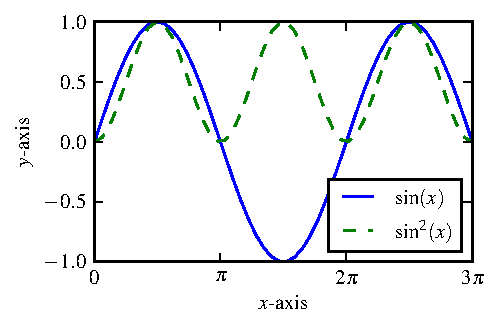
\includegraphics[width=\columnwidth]{myplot.pdf}\hfill}
\caption{A matplotlib plot created with PythonTeX. \DUrole{label}{mplfig}}
\end{figure}


\subsection{Solving equations with NumPy%
  \label{solving-equations-with-numpy}%
}


PythonTeX didn't require any special modifications to the Python
code in the previous example with matplotlib.
The code that created the plot was the same as it would
have been had an external script been used to generate the plot.  In some
situations, however, it can be beneficial to acknowledge the LaTeX context
of the Python code.  This may be illustrated by solving an equation with
NumPy \cite{NP}.

Perhaps the most obvious way to solve an equation using PythonTeX is to
separate the Python solving from the LaTeX typesetting.  Consider finding
the roots of a polynomial using NumPy.\begin{Verbatim}[commandchars=\\\{\},fontsize=\footnotesize]
\PY{k}{\PYZbs{}begin}\PY{n+nb}{\PYZob{}}pylabcode\PY{n+nb}{\PYZcb{}}
coeff = [4, 2, -4]
r = roots(coeff)
\PY{k}{\PYZbs{}end}\PY{n+nb}{\PYZob{}}pylabcode\PY{n+nb}{\PYZcb{}}

The roots of \PY{l+s}{\PYZdl{}}\PY{l+m}{4}\PY{n+nb}{x}\PY{n+nb}{\PYZca{}}\PY{l+m}{2}\PY{n+nb}{ }\PY{o}{+}\PY{n+nb}{ }\PY{l+m}{2}\PY{n+nb}{x }\PY{o}{-}\PY{n+nb}{ }\PY{l+m}{4}\PY{n+nb}{ }\PY{o}{=}\PY{n+nb}{ }\PY{l+m}{0}\PY{l+s}{\PYZdl{}} are
\PY{l+s}{\PYZdl{}}\PY{n+nv}{\PYZbs{}pylab}\PY{n+nb}{\PYZob{}}\PY{n+nb}{r}\PY{o}{[}\PY{l+m}{0}\PY{o}{]}\PY{n+nb}{\PYZcb{}}\PY{l+s}{\PYZdl{}} and \PY{l+s}{\PYZdl{}}\PY{n+nv}{\PYZbs{}pylab}\PY{n+nb}{\PYZob{}}\PY{n+nb}{r}\PY{o}{[}\PY{l+m}{1}\PY{o}{]}\PY{n+nb}{\PYZcb{}}\PY{l+s}{\PYZdl{}}.
\end{Verbatim}
This yields\begin{quotation}%
\begin{quote}


The roots of $4x^2 + 2x - 4 = 0$ are
$-1.2807764064$ and $0.780776406404$.
\end{quote}
\end{quotation}

Such an approach works, but the code must be modified significantly whenever
the polynomial changes.  A more sophisticated approach automatically
generates the LaTeX code and perhaps rounds the roots as well, for an
arbitrary polynomial.\begin{Verbatim}[commandchars=\\\{\},fontsize=\footnotesize]
\PY{k}{\PYZbs{}begin}\PY{n+nb}{\PYZob{}}pylabcode\PY{n+nb}{\PYZcb{}}
coeff = [4, 2, -4]
\PYZsh{} Build a string containing equation
eq = ''
for n, c in enumerate(coeff):
    if n == 0 or str(c).startswith('-'):
        eq += str(c)
    else:
        eq += '+' + str(c)
    if len(coeff) - n - 1 == 1:
        eq += 'x'
    elif len(coeff) - n - 1 \PYZgt{} 1:
        eq += 'x\PY{n+nb}{\PYZca{}}' + str(len(coeff) - n - 1)
eq += '=0'
\PYZsh{} Get roots and format for LaTeX
r = ['\PY{n+nb}{\PYZob{}}0:+.3f\PY{n+nb}{\PYZcb{}}'.format(root)
  for root in roots(coeff)]
latex\PY{n+nb}{\PYZus{}}roots = ','.join(r)
\PY{k}{\PYZbs{}end}\PY{n+nb}{\PYZob{}}pylabcode\PY{n+nb}{\PYZcb{}}

The roots of \PY{l+s}{\PYZdl{}}\PY{n+nv}{\PYZbs{}pylab}\PY{n+nb}{\PYZob{}}\PY{n+nb}{eq}\PY{n+nb}{\PYZcb{}}\PY{l+s}{\PYZdl{}} are
\PY{l+s}{\PYZdl{}}\PY{o}{[}\PY{n+nv}{\PYZbs{}pylab}\PY{n+nb}{\PYZob{}}\PY{n+nb}{latex}\PY{n+nb}{\PYZus{}}\PY{n+nb}{roots}\PY{n+nb}{\PYZcb{}}\PY{o}{]}\PY{l+s}{\PYZdl{}}.
\end{Verbatim}
This yields\begin{quotation}%
\begin{quote}


The roots of $4x^2+2x-4=0$ are
$[-1.281,+0.781]$.
\end{quote}
\end{quotation}
% 


The automated generation of LaTeX code on the Python side begins to
demonstrate the full power of PythonTeX.

\subsection{Solving equations with SymPy%
  \label{solving-equations-with-sympy}%
}


Several examples with SymPy further illustrate the potential of Python-generated LaTeX code \cite{SymPy}.

To simplify SymPy use, PythonTeX provides a set of commands and
environments that begin with the prefix \texttt{sympy}.  These are
identical to their \texttt{py} counterparts, except that SymPy is
automatically imported via \texttt{from sympy import *}.

SymPy is ideal for PythonTeX use, because its \texttt{LatexPrinter} class and the associated \texttt{latex()} function provide LaTeX representations of objects.  For example, returning to solving the same polynomial,\begin{Verbatim}[commandchars=\\\{\},fontsize=\footnotesize]
\PY{k}{\PYZbs{}begin}\PY{n+nb}{\PYZob{}}sympycode\PY{n+nb}{\PYZcb{}}
x = symbols('x')
myeq = Eq(4*x**2 + 2*x - 4)
print('The roots of the equation ')
print(latex(myeq, mode='inline'))
print(' are ')
print(latex(solve(myeq), mode='inline'))
\PY{k}{\PYZbs{}end}\PY{n+nb}{\PYZob{}}sympycode\PY{n+nb}{\PYZcb{}}
\end{Verbatim}
creates\begin{quotation}%
\begin{quote}


The roots of the equation $4 x^{2} + 2 x -4 = 0$
are $\begin{bmatrix}- \frac{1}{4} \sqrt{17} - \frac{1}{4},
& - \frac{1}{4} + \frac{1}{4} \sqrt{17}\end{bmatrix}$
\end{quote}
\end{quotation}

Notice that the printed content appears as a single uninterrupted line,
even though it was produced by multiple prints.  This is because
the printed content is interpreted as LaTeX code, and in LaTeX an empty
line is required to end a paragraph.

The \texttt{\textbackslash{}sympy} command provides an alternative to printing.
While the \texttt{\textbackslash{}py} and \texttt{\textbackslash{}pylab} commands attempt to convert
their arguments directly to a string, the \texttt{\textbackslash{}sympy} command converts its
argument using SymPy's \texttt{LatexPrinter} class.  Thus, the output from the
last example could also have been produced using\begin{Verbatim}[commandchars=\\\{\},fontsize=\footnotesize]
\PY{k}{\PYZbs{}begin}\PY{n+nb}{\PYZob{}}sympycode\PY{n+nb}{\PYZcb{}}
x = symbols('x')
myeq = Eq(4*x**2 + 2*x - 4)
\PY{k}{\PYZbs{}end}\PY{n+nb}{\PYZob{}}sympycode\PY{n+nb}{\PYZcb{}}

The roots of the equation \PY{l+s}{\PYZdl{}}\PY{n+nv}{\PYZbs{}sympy}\PY{n+nb}{\PYZob{}}\PY{n+nb}{myeq}\PY{n+nb}{\PYZcb{}}\PY{l+s}{\PYZdl{}}
are \PY{l+s}{\PYZdl{}}\PY{n+nv}{\PYZbs{}sympy}\PY{n+nb}{\PYZob{}}\PY{n+nb}{solve}\PY{o}{(}\PY{n+nb}{myeq}\PY{o}{)}\PY{n+nb}{\PYZcb{}}\PY{l+s}{\PYZdl{}}.
\end{Verbatim}

% 
The \texttt{\textbackslash{}sympy} command uses a special interface to the \texttt{LatexPrinter} class,
to allow for context-dependent \texttt{LatexPrinter} settings.  PythonTeX includes
a utilities class, and an instance of this class called \texttt{pytex} is
created within each PythonTeX session.  The \texttt{formatter()} method of
this class is responsible for converting objects into strings for \texttt{\textbackslash{}py},
\texttt{\textbackslash{}pylab}, and \texttt{\textbackslash{}sympy}.  In the case of SymPy, \texttt{pytex.formatter()}
provides an interface to \texttt{LatexPrinter}, with provision for context-dependent
customization.  In LaTeX, there are four possible math styles:  displaystyle
(regular equations), textstyle (inline), scriptstyle (superscripts and
subscripts), and scriptscriptstyle (superscripts and subscripts, of
superscripts and subscripts).  Separate \texttt{LatexPrinter} settings may be
specified for each of these styles individually, using a command of the form%
\begin{quote}\begin{verbatim}
pytex.set_sympy_latex(style, **kwargs)
\end{verbatim}

\end{quote}
For example, by default \texttt{\textbackslash{}sympy} is set to create normal-sized matrices
in displaystyle and small matrices elsewhere.  Thus, the following code\begin{Verbatim}[commandchars=\\\{\},fontsize=\footnotesize]
\PY{k}{\PYZbs{}begin}\PY{n+nb}{\PYZob{}}sympycode\PY{n+nb}{\PYZcb{}}
m = Matrix([[1,0], [0,1]])
\PY{k}{\PYZbs{}end}\PY{n+nb}{\PYZob{}}sympycode\PY{n+nb}{\PYZcb{}}

The matrix in inline is small:  \PY{l+s}{\PYZdl{}}\PY{n+nv}{\PYZbs{}sympy}\PY{n+nb}{\PYZob{}}\PY{n+nb}{m}\PY{n+nb}{\PYZcb{}}\PY{l+s}{\PYZdl{}}

The matrix in an equation is of normal size:
\PY{l+s+sb}{\PYZbs{}[}\PY{n+nb}{ }\PY{n+nv}{\PYZbs{}sympy}\PY{n+nb}{\PYZob{}}\PY{n+nb}{m}\PY{n+nb}{\PYZcb{}}\PY{n+nb}{ }\PY{l+s}{\PYZbs{}]}
\end{Verbatim}
produces\begin{quotation}%
\begin{quote}


The matrix in inline is small:
$\mathchoice{\begin{pmatrix}1 & 0\\0 &
1\end{pmatrix}}{\left(\begin{smallmatrix}1 & 0\\0 &
1\end{smallmatrix}\right)}{\left(\begin{smallmatrix}1 & 0\\0 &
1\end{smallmatrix}\right)}{\left(\begin{smallmatrix}1 & 0\\0 &
1\end{smallmatrix}\right)}$

The matrix in an equation is
of normal size:\begin{equation*}
\mathchoice{\begin{pmatrix}1 & 0\\0 &
1\end{pmatrix}}{\left(\begin{smallmatrix}1 & 0\\0 &
1\end{smallmatrix}\right)}{\left(\begin{smallmatrix}1 & 0\\0 &
1\end{smallmatrix}\right)}{\left(\begin{smallmatrix}1 & 0\\0 &
1\end{smallmatrix}\right)}
\end{equation*}
\end{quote}
\end{quotation}
% 

% 
As another example, consider customizing the appearance of inverse
trigonometric functions based on their context.\begin{Verbatim}[commandchars=\\\{\},fontsize=\footnotesize]
\PY{k}{\PYZbs{}begin}\PY{n+nb}{\PYZob{}}sympycode\PY{n+nb}{\PYZcb{}}
x = symbols('x')
sineq = Eq(asin(x/2)-pi/3)
pytex.set\PY{n+nb}{\PYZus{}}sympy\PY{n+nb}{\PYZus{}}latex('display',
                      inv\PY{n+nb}{\PYZus{}}trig\PY{n+nb}{\PYZus{}}style='power')
pytex.set\PY{n+nb}{\PYZus{}}sympy\PY{n+nb}{\PYZus{}}latex('text',
                      inv\PY{n+nb}{\PYZus{}}trig\PY{n+nb}{\PYZus{}}style='full')
\PY{k}{\PYZbs{}end}\PY{n+nb}{\PYZob{}}sympycode\PY{n+nb}{\PYZcb{}}

Inline:  \PY{l+s}{\PYZdl{}}\PY{n+nv}{\PYZbs{}sympy}\PY{n+nb}{\PYZob{}}\PY{n+nb}{sineq}\PY{n+nb}{\PYZcb{}}\PY{l+s}{\PYZdl{}}

Equation:  \PY{l+s+sb}{\PYZbs{}[}\PY{n+nb}{ }\PY{n+nv}{\PYZbs{}sympy}\PY{n+nb}{\PYZob{}}\PY{n+nb}{sineq}\PY{n+nb}{\PYZcb{}}\PY{n+nb}{ }\PY{l+s}{\PYZbs{}]}
\end{Verbatim}
This creates\begin{quotation}%
\begin{quote}


Inline:  $\mathchoice{\operatorname{sin}^{-1}\left(\frac{1}{2} x\right) -
\frac{1}{3} \pi = 0}{\operatorname{arcsin}\left(\frac{1}{2} x\right) -
\frac{1}{3} \pi = 0}{\operatorname{arcsin}\left(\frac{1}{2} x\right) -
\frac{1}{3} \pi = 0}{\operatorname{arcsin}\left(\frac{1}{2} x\right) -
\frac{1}{3} \pi = 0}$

Equation:\begin{equation*}
\mathchoice{\operatorname{sin}^{-1}\left(\frac{1}{2} x\right) -
\frac{1}{3} \pi = 0}{\operatorname{arcsin}\left(\frac{1}{2} x\right) -
\frac{1}{3} \pi = 0}{\operatorname{arcsin}\left(\frac{1}{2} x\right) -
\frac{1}{3} \pi = 0}{\operatorname{arcsin}\left(\frac{1}{2} x\right) -
\frac{1}{3} \pi = 0}
\end{equation*}
\end{quote}
\end{quotation}
% 

% 
Notice that in both examples above, the \texttt{\textbackslash{}sympy} command is simply used—no
information about context must be passed to Python.  On the Python side, the
context-dependent \texttt{LatexPrinter} settings are used to determine whether the LaTeX
representation of some object is context-dependent.  If not, Python creates a
single LaTeX representation of the object and returns that.  If the LaTeX
representation is context-dependent, then Python returns multiple LaTeX
representations, wrapped in LaTeX's \texttt{\textbackslash{}mathchoice} macro.  The
\texttt{\textbackslash{}mathchoice} macro takes four arguments, one for each of the four LaTeX
math styles display, text, script, and scriptscript.  The correct argument
is typeset by LaTeX based on the current math style.

\subsection{Step-by-step derivations with SymPy%
  \label{step-by-step-derivations-with-sympy}%
}


With SymPy's LaTeX functionality, it is simple to automate tasks that
could otherwise be tedious.  Instead of manually typing
step-by-step mathematical solutions, or copying them from an external
program, the user can generate them automatically from within LaTeX.\begin{Verbatim}[commandchars=\\\{\},fontsize=\footnotesize]
\PY{k}{\PYZbs{}begin}\PY{n+nb}{\PYZob{}}sympycode\PY{n+nb}{\PYZcb{}}
x, y = symbols('x, y')
f = x + sin(y)
step1 = Integral(f, x, y)
step2 = Integral(Integral(f, x).doit(), y)
step3 = step2.doit()
\PY{k}{\PYZbs{}end}\PY{n+nb}{\PYZob{}}sympycode\PY{n+nb}{\PYZcb{}}

\PY{k}{\PYZbs{}begin}\PY{n+nb}{\PYZob{}}align*\PY{n+nb}{\PYZcb{}}
\PY{k}{\PYZbs{}sympy}\PY{n+nb}{\PYZob{}}step1\PY{n+nb}{\PYZcb{}} \PY{n+nb}{\PYZam{}}= \PY{k}{\PYZbs{}sympy}\PY{n+nb}{\PYZob{}}step2\PY{n+nb}{\PYZcb{}} \PY{k}{\PYZbs{}\PYZbs{}}
              \PY{n+nb}{\PYZam{}}= \PY{k}{\PYZbs{}sympy}\PY{n+nb}{\PYZob{}}step3\PY{n+nb}{\PYZcb{}}
\PY{k}{\PYZbs{}end}\PY{n+nb}{\PYZob{}}align*\PY{n+nb}{\PYZcb{}}
\end{Verbatim}
This produces\begin{quotation}%
\begin{quote}
\begin{align*}
\iint x + \operatorname{sin}\left(y\right)\, dx\, dy
&= \int \frac{1}{2} x^{2} + x \operatorname{sin}\left(y\right)\, dy \\
&= \frac{1}{2} x^{2} y - x \operatorname{cos}\left(y\right)
\end{align*}
\end{quote}
\end{quotation}
% 

% 


\subsection{Automated mathematical tables with SymPy%
  \label{automated-mathematical-tables-with-sympy}%
}
The creation of mathematical tables is another traditionally tedious task
that may be automated with PythonTeX and SymPy.  Consider the following
code, which automatically creates a small integral and derivative table.\begin{Verbatim}[commandchars=\\\{\},fontsize=\footnotesize]
\PY{k}{\PYZbs{}begin}\PY{n+nb}{\PYZob{}}sympycode\PY{n+nb}{\PYZcb{}}
x = symbols('x')
funcs = ['sin(x)', 'cos(x)', 'sinh(x)', 'cosh(x)']
ops = ['Integral', 'Derivative']
print('\PY{k}{\PYZbs{}\PYZbs{}}begin\PY{n+nb}{\PYZob{}}align*\PY{n+nb}{\PYZcb{}}')
for func in funcs:
    for op in ops:
        obj = eval(op + '(' + func + ', x)')
        left = latex(obj)
        right = latex(obj.doit())
        if op != ops[-1]:
            print(left + '\PY{n+nb}{\PYZam{}}=' + right + '\PY{n+nb}{\PYZam{}}')
        else:
            print(left + '\PY{n+nb}{\PYZam{}}=' + right + r'\PY{k}{\PYZbs{}\PYZbs{}}')
print('\PY{k}{\PYZbs{}\PYZbs{}}end\PY{n+nb}{\PYZob{}}align*\PY{n+nb}{\PYZcb{}}')
\PY{k}{\PYZbs{}end}\PY{n+nb}{\PYZob{}}sympycode\PY{n+nb}{\PYZcb{}}
\end{Verbatim}
\begin{align*}
\int \operatorname{sin}\left(x\right)\, dx&=- \operatorname{cos}\left(x\right)&
\frac{\partial}{\partial x} \operatorname{sin}\left(x\right)&=\operatorname{cos}\left(x\right)\\
\int \operatorname{cos}\left(x\right)\, dx&=\operatorname{sin}\left(x\right)&
\frac{\partial}{\partial x} \operatorname{cos}\left(x\right)&=- \operatorname{sin}\left(x\right)\\
\int \operatorname{sinh}\left(x\right)\, dx&=\operatorname{cosh}\left(x\right)&
\frac{\partial}{\partial x} \operatorname{sinh}\left(x\right)&=\operatorname{cosh}\left(x\right)\\
\int \operatorname{cosh}\left(x\right)\, dx&=\operatorname{sinh}\left(x\right)&
\frac{\partial}{\partial x} \operatorname{cosh}\left(x\right)&=\operatorname{sinh}\left(x\right)\\
\end{align*}
% 

% 
This code could easily be modified to generate a page or more of integrals
and derivatives by simply adding additional function names to the \texttt{funcs} list.

\subsection{Debugging and access to stderr%
  \label{debugging-and-access-to-stderr}%
}


PythonTeX commands and environments save the Python code they contain
to an external file, where it is processed by PythonTeX.  When the
Python code is executed, errors may occur.  The line numbers for these
errors do not correspond to the document line numbers, because only the
Python code contained in the document is executed; the LaTeX code is not
present.  Furthermore, the error line numbers do not correspond to the
line numbers that would be obtained by only counting the Python code
in the document, because PythonTeX must execute some boilerplate
management code in addition to the user's code.  This presents a challenge
for debugging.

PythonTeX addresses this issue by tracking the original LaTeX document
line number for each piece of code.  All error messages are parsed, and
Python code line numbers are converted to LaTeX document line numbers.
The raw stderr from the Python code is interspersed with PythonTeX
messages giving the document line numbers.  For example, consider the
following code, with a syntax error in the last line:\begin{Verbatim}[commandchars=\\\{\},fontsize=\footnotesize]
\PY{k}{\PYZbs{}begin}\PY{n+nb}{\PYZob{}}pyblock\PY{n+nb}{\PYZcb{}}[errorsession]
x = 1
y = 2
z = x + y +
\PY{k}{\PYZbs{}end}\PY{n+nb}{\PYZob{}}pyblock\PY{n+nb}{\PYZcb{}}
\end{Verbatim}
The error occurred on line 3 of the Python code, but this might be line
104 of the actual document and line 47 of the combined code and
boilerplate.  In this case, running the PythonTeX script that processes
Python code would produce the following message, where \texttt{<temp file name>}
would be the name of a temporary file that was executed:%
\begin{quote}\begin{verbatim}
* PythonTeX code error on line 104:
    File "<temp file name>", line 47
      z = x + y +
                ^
  SyntaxError: invalid syntax
\end{verbatim}

\end{quote}
Thus, finding code error locations is as simple as it would be if
the code were written in separate files and executed individually.
PythonTeX is the first Python-LaTeX solution to provide such
comprehensive error line synchronization.

In general, errors are something to avoid.  In the context of writing
about code, however, they may be created intentionally for instructional
purposes.  Thus, PythonTeX also provides access to error messages in a
form suitable for typesetting.  If the PythonTeX package option \texttt{stderr}
is enabled, any error message created by the most recent PythonTeX command
or environment is available via \texttt{\textbackslash{}stderrpythontex}.  By default, stderr
content is brought in as LaTeX verbatim content; this preserves formatting
and prevents issues caused by stderr content not being valid LaTeX.

Python code and the error it produces may be typeset next to
each other.  Reusing the previous example,\begin{Verbatim}[commandchars=\\\{\},fontsize=\footnotesize]
\PY{k}{\PYZbs{}begin}\PY{n+nb}{\PYZob{}}pyblock\PY{n+nb}{\PYZcb{}}[errorsession]
x = 1
y = 2
z = x + y +
\PY{k}{\PYZbs{}end}\PY{n+nb}{\PYZob{}}pyblock\PY{n+nb}{\PYZcb{}}
\end{Verbatim}
creates the following typeset code:\begin{Verbatim}[commandchars=\\\{\},fontsize=\footnotesize]
\PY{n}{x} \PY{o}{=} \PY{l+m+mi}{1}
\PY{n}{y} \PY{o}{=} \PY{l+m+mi}{2}
\PY{n}{z} \PY{o}{=} \PY{n}{x} \PY{o}{+} \PY{n}{y} \PY{o}{+}
\end{Verbatim}
The stderr may be brought in via \texttt{\textbackslash{}stderrpythontex}:%
\begin{quote}\begin{verbatim}
  File "<file>", line 3
    z = x + y +
              ^
SyntaxError: invalid syntax
\end{verbatim}

\end{quote}

% 
Two things are noteworthy about the form of the stderr.  First, in the
case shown, the file name is given as \texttt{"<file>"}.  PythonTeX provides
a package option \texttt{stderrfilename} for controlling this name.  The
actual name of the temporary file that was executed may be shown, or
simply a name based on the session (\texttt{"errorsession.py"} in this case), or the
more generic \texttt{"<file>"} or \texttt{"<script>"}.  Second, the line number
shown corresponds to the code that was actually entered in the document,
not to the document line number or to the line number of the code that
was actually executed (which would have included PythonTeX boilerplate).
To accomplish this, PythonTeX parses the stderr and corrects the line
number, so that the typeset code and the typeset stderr are in sync.

\subsection{General code highlighting with Pygments%
  \label{general-code-highlighting-with-pygments}%
}


The primary purpose of PythonTeX is to execute Python code included in
LaTeX documents and provide access to the output.  Once support for
Pygments highlighting of Python code was added \cite{Pyg}, however, it was simple
to add support for general code highlighting.

PythonTeX provides a \texttt{\textbackslash{}pygment} command for typesetting inline code
snippets, a \texttt{pygments} environment for typesetting blocks of code,
and an \texttt{\textbackslash{}inputpygments} command for bringing in and highlighting an
external file.  All of these have a mandatory argument that
specifies the Pygments lexer to be used.  For example, \texttt{\textbackslash{}pygment\{latex\}\{\textbackslash{}pygment\}} produces\begin{Verbatim}[commandchars=\\\{\},fontsize=\footnotesize]
\PY{k}{\PYZbs{}pygment}
\end{Verbatim}
in a form suitable for inline use while\begin{Verbatim}[commandchars=\\\{\},fontsize=\footnotesize]
\PY{k}{\PYZbs{}begin}\PY{n+nb}{\PYZob{}}pygments\PY{n+nb}{\PYZcb{}}\PY{n+nb}{\PYZob{}}python\PY{n+nb}{\PYZcb{}}
def f(x):
    return x**3
\PY{k}{\PYZbs{}end}\PY{n+nb}{\PYZob{}}pygments\PY{n+nb}{\PYZcb{}}
\end{Verbatim}
creates\begin{Verbatim}[commandchars=\\\{\},fontsize=\footnotesize]
\PY{k}{def} \PY{n+nf}{f}\PY{p}{(}\PY{n}{x}\PY{p}{)}\PY{p}{:}
    \PY{k}{return} \PY{n}{x}\PY{o}{*}\PY{o}{*}\PY{l+m+mi}{3}
\end{Verbatim}
The \texttt{pygments} environment and the \texttt{\textbackslash{}inputpygments} command
accept an optional argument containing \texttt{fancyvrb} settings.

As far as the author is aware, PythonTeX is the only LaTeX package that
provides Pygments highlighting with Unicode support under the
standard pdfTeX engine.  The \texttt{listings} package \cite{LST}, probably the
most prominent non-Pygments highlighting package, does support
Unicode—but only if the user follows special procedures that could
become tedious.  PythonTeX requires no special treatment of Unicode
characters, so long as the \texttt{fontenc} and \texttt{inputenc} packages
are loaded and used correctly.  For example, PythonTeX can correctly
highlight the following snippet copied and pasted from a Python 3
console session, without any modification.\begin{Verbatim}[commandchars=\\\{\},fontsize=\footnotesize]
\PY{g+gp}{\PYZgt{}\PYZgt{}\PYZgt{} }\PY{n}{var1} \PY{o}{=} \PY{l+s}{'}\PY{l+s}{âæéöø}\PY{l+s}{'}
\PY{g+gp}{\PYZgt{}\PYZgt{}\PYZgt{} }\PY{n}{var2} \PY{o}{=} \PY{l+s}{'}\PY{l+s}{ßçñðŠ}\PY{l+s}{'}
\PY{g+gp}{\PYZgt{}\PYZgt{}\PYZgt{} }\PY{n}{var1} \PY{o}{+} \PY{n}{var2}
\PY{g+go}{'âæéöøßçñðŠ'}
\end{Verbatim}

% 


\subsection{Implementation%
  \label{implementation}%
}
A brief overview of the internal workings of PythonTeX is provided
below.  For additional details, please consult the documentation.

When a LaTeX document is compiled, the PythonTeX commands and environments
write their contents to a single shared external file.  The command and
environment contents are interspersed with delimiters, which contain
information about the type
of command or environment, the session in which the code is to be
executed, the document line number where the code originated, and
similar tracking information.  A single external file is used
to minimize the number of temporary files created, and because TeX
has a very limited number of output streams.

During compilation, each command and environment also checks for any Python-generated content that belongs to it, and brings in this content
if it exists.  Python-generated content is brought in via LaTeX macros
and via separate external files.  At the beginning of the LaTeX document,
the PythonTeX package brings in two files of LaTeX macros that were
created on the Python side, if these files exist.  One file consists
of macros containing the Python content accessed by \texttt{\textbackslash{}py}, \texttt{\textbackslash{}pylab},
and \texttt{\textbackslash{}sympy}.  The other file contains highlighted Pygments content.
The files are separate for performance reasons.  In addition to content
that is brought in via macros, content may be brought in via separate
external files.  Each command or environment that uses the print
statement/function must bring in an external file containing the
printed content.  The printed content cannot be brought in as LaTeX
macros, because in general printed content need not be valid LaTeX
code.  In contrast, \texttt{\textbackslash{}py}, \texttt{\textbackslash{}pylab}, and \texttt{\textbackslash{}sympy} should return valid
LaTeX, and of course Pygments-highlighted content is valid LaTeX
as well.

On the Python side, the file containing code and delimiters must be
processed.  All code is hashed, to determine what has been modified
since the previous run so that only new and modified code may be
executed.  Code that must be executed is divided by session, and each
session (plus some PythonTeX management code) is saved to its own
external file.  The highlighting settings for Pygments content are
compared with the settings for the last run, to determine what needs
to be highlighted again with new settings.

Next, Python's \texttt{multiprocessing} package is used to perform all
necessary tasks.  Each of the session code files is executed within
a separate process.  The process executes the file, parses the stdout
into separate files of printed content based on the command or
environment from which it originated, and parses the stderr to
synchronize it with the document line numbers.  If specified by the
user, a modified version of the stderr is created and saved in an
external file for inclusion in the document via \texttt{\textbackslash{}stderrpythontex}.
Two additional processes are used, one for highlighting code with
Pygments and one for evaluating and highlighting all console content
(using Python's \texttt{code} module).

Finally, all LaTeX macros created by all processes are saved in
one of two external files, depending on whether they contain general
content or content highlighted by Pygments (again, this is for
performance reasons).  All information that will be needed the next
time the Python side runs is saved.  This includes the hashes for
each session.  Any session that produced errors is automatically set
to be executed the next time the Python side runs.  A list of all files
that were automatically created by PythonTeX is also saved, so
that future runs can clean up outdated and unused files.

PythonTeX consists of a LaTeX package and several Python scripts.
A complete compilation cycle for a PythonTeX document involves running
LaTeX to create the file of code and delimiters, running the PythonTeX
script to create Python content, and finally running LaTeX again
to compile the document with Python-generated content included.  Since
all Python-generated content is saved, the PythonTeX script only needs
to be run when the document's PythonTeX commands or environments are
modified.  By default, all files created by PythonTeX are kept in a
subdirectory within the document directory, keeping things tidy.

\subsection{Conclusion%
  \label{conclusion}%
}


PythonTeX provides access to the full power of Python from within
LaTeX documents.  This can greatly simplify the creation of scientific
documents and presentations.

One of the potential drawbacks of using a special LaTeX package
like PythonTeX is that publishers may not support it.  Since PythonTeX
saves all Python-generated content, it already provides document
compilation without the execution of any Python code, so that aspect will
not be an issue.  Ideally, a PythonTeX document and its Python output
could be merged into a single, new document that does not require the
PythonTeX package.  This feature is being considered for an upcoming release.

PythonTeX provides many features not discussed here, including
a number of formatting options and methods for adding custom code to
all sessions.  PythonTeX is also under active
development.  For additional information and the latest code,
please visit \url{https://github.com/gpoore/pythontex}.
\begin{thebibliography}{SympyTeX}
\bibitem[Sweave]{Sweave}{

F. Leisch. \emph{Sweave: Dynamic generation of statistical reports
using literate data analysis}, in Wolfgang Härdle and Bernd Rönz,
editors, Compstat 2002 - Proceedings in Computational Statistics,
pages 575-580. Physica Verlag, Heidelberg, 2002. ISBN 3-7908-1517-9.
\url{http://www.statistik.lmu.de/~leisch/Sweave/}}
\bibitem[Ehmsen]{Ehmsen}{

M. R. Ehmsen.  ``Python in LaTeX.''
\url{http://web.archive.org/web/20080728170129/www.imada.sdu.dk/~ehmsen/python.sty}}
\bibitem[SageTeX]{SageTeX}{

D. Drake. ``The SageTeX package.''
\url{https://bitbucket.org/ddrake/sagetex/}}
\bibitem[SympyTeX]{SympyTeX}{

T. Molteno. ``The sympytex package.''
\url{https://github.com/tmolteno/SympyTeX/}}
\bibitem[SymPy]{SymPy}{

SymPy Development Team. ``SymPy.'' \url{http://sympy.org/}}
\bibitem[Pyg]{Pyg}{

The Pocoo Team. ``Pygments: Python Syntax Highlighter.''
\url{http://pygments.org/}}
\bibitem[FV]{FV}{

T. Van Zandt, D. Girou, S. Rahtz, and H. Voß.  ``The 'fancyvrb'
package:  Fancy Verbatims in LaTeX.'' \url{http://www.ctan.org/pkg/fancyvrb}}
\bibitem[MPL]{MPL}{

J. D. Hunter. \emph{Matplotlib: A 2D Graphics Environment}, in Computing in
Science \& Engineering, Vol. 9, No. 3. (2007), pp. 90-95.
\url{http://matplotlib.sourceforge.net/}}
\bibitem[NP]{NP}{

Numpy developers.  ``NumPy.''  \url{http://numpy.scipy.org/}}
\bibitem[LST]{LST}{

C. Heinz and B. Moses.  ``The Listings Package.''
\url{http://www.ctan.org/tex-archive/macros/latex/contrib/listings/}}
\end{thebibliography}

\end{document}
